\section{4+1 Architectural View Model}


In this section we will describe the \gls{app} using the 4+1 Architectural View Model. With this model we will represent
the \gls{app} using five different views, which should focus on specific elements of the project. Each view provide
a different purpose \cite{refart:KR41}. For this project we will provide the 3 following views of the 4+1 Architectural View 
Model:

\begin{itemize}
    \item \textbf{Scenario view}: simple description for the end user 
    \item \textbf{Behaviour view}: description of the existing processes
    \item \textbf{Structural view}: object-oriented decomposition
\end{itemize}

The scenario view was presented in the section \ref{Primary_Functionality} of this project.

\newpage
\subsection{Behaviour view}
The following \gls{activity diagram} depicts the register and login procedure within the app.

\begin{figure}[H]
    \centering
    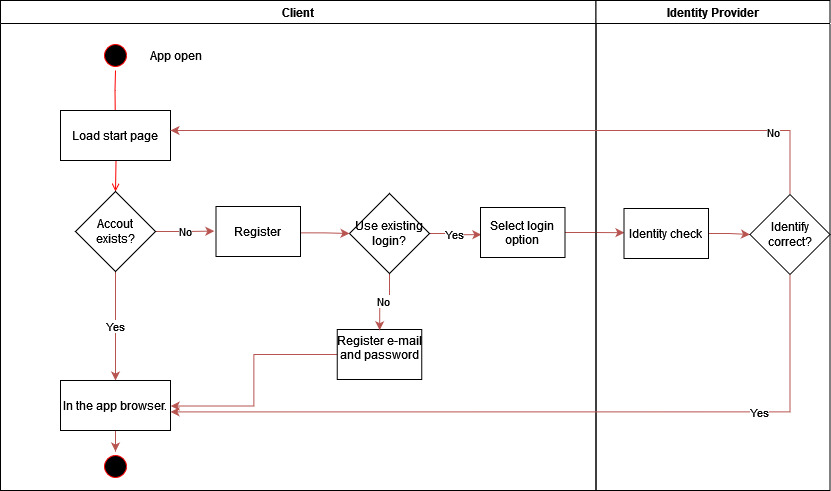
\includegraphics[width=1\textwidth]{assets/login_AC.jpg}
    \caption{Login procedures}
    \label{fig:login_register}
\end{figure}

\newpage
\subsection{Structural view}
To describe this view we choose a \gls{class diagram}. With it we may provide a static description of elements
within the structure of our system. They can also be used during the programming process to display what is needed
to be done.

\begin{figure}[H]
    \centering
    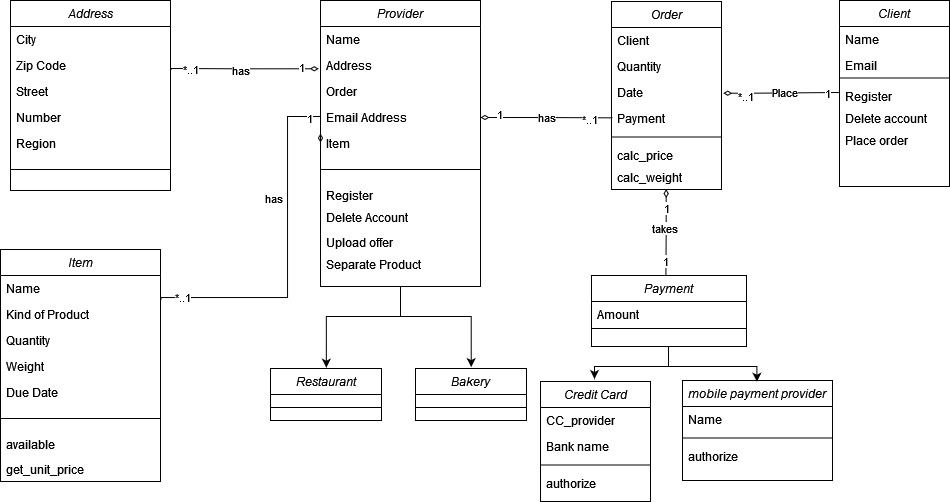
\includegraphics[width=1\textwidth]{assets/classes_CD.jpg}
    \caption{Classes of the project}
    \label{fig:class_CD}
\end{figure}
 


